\begin{figure}[htbp]
  \centering
  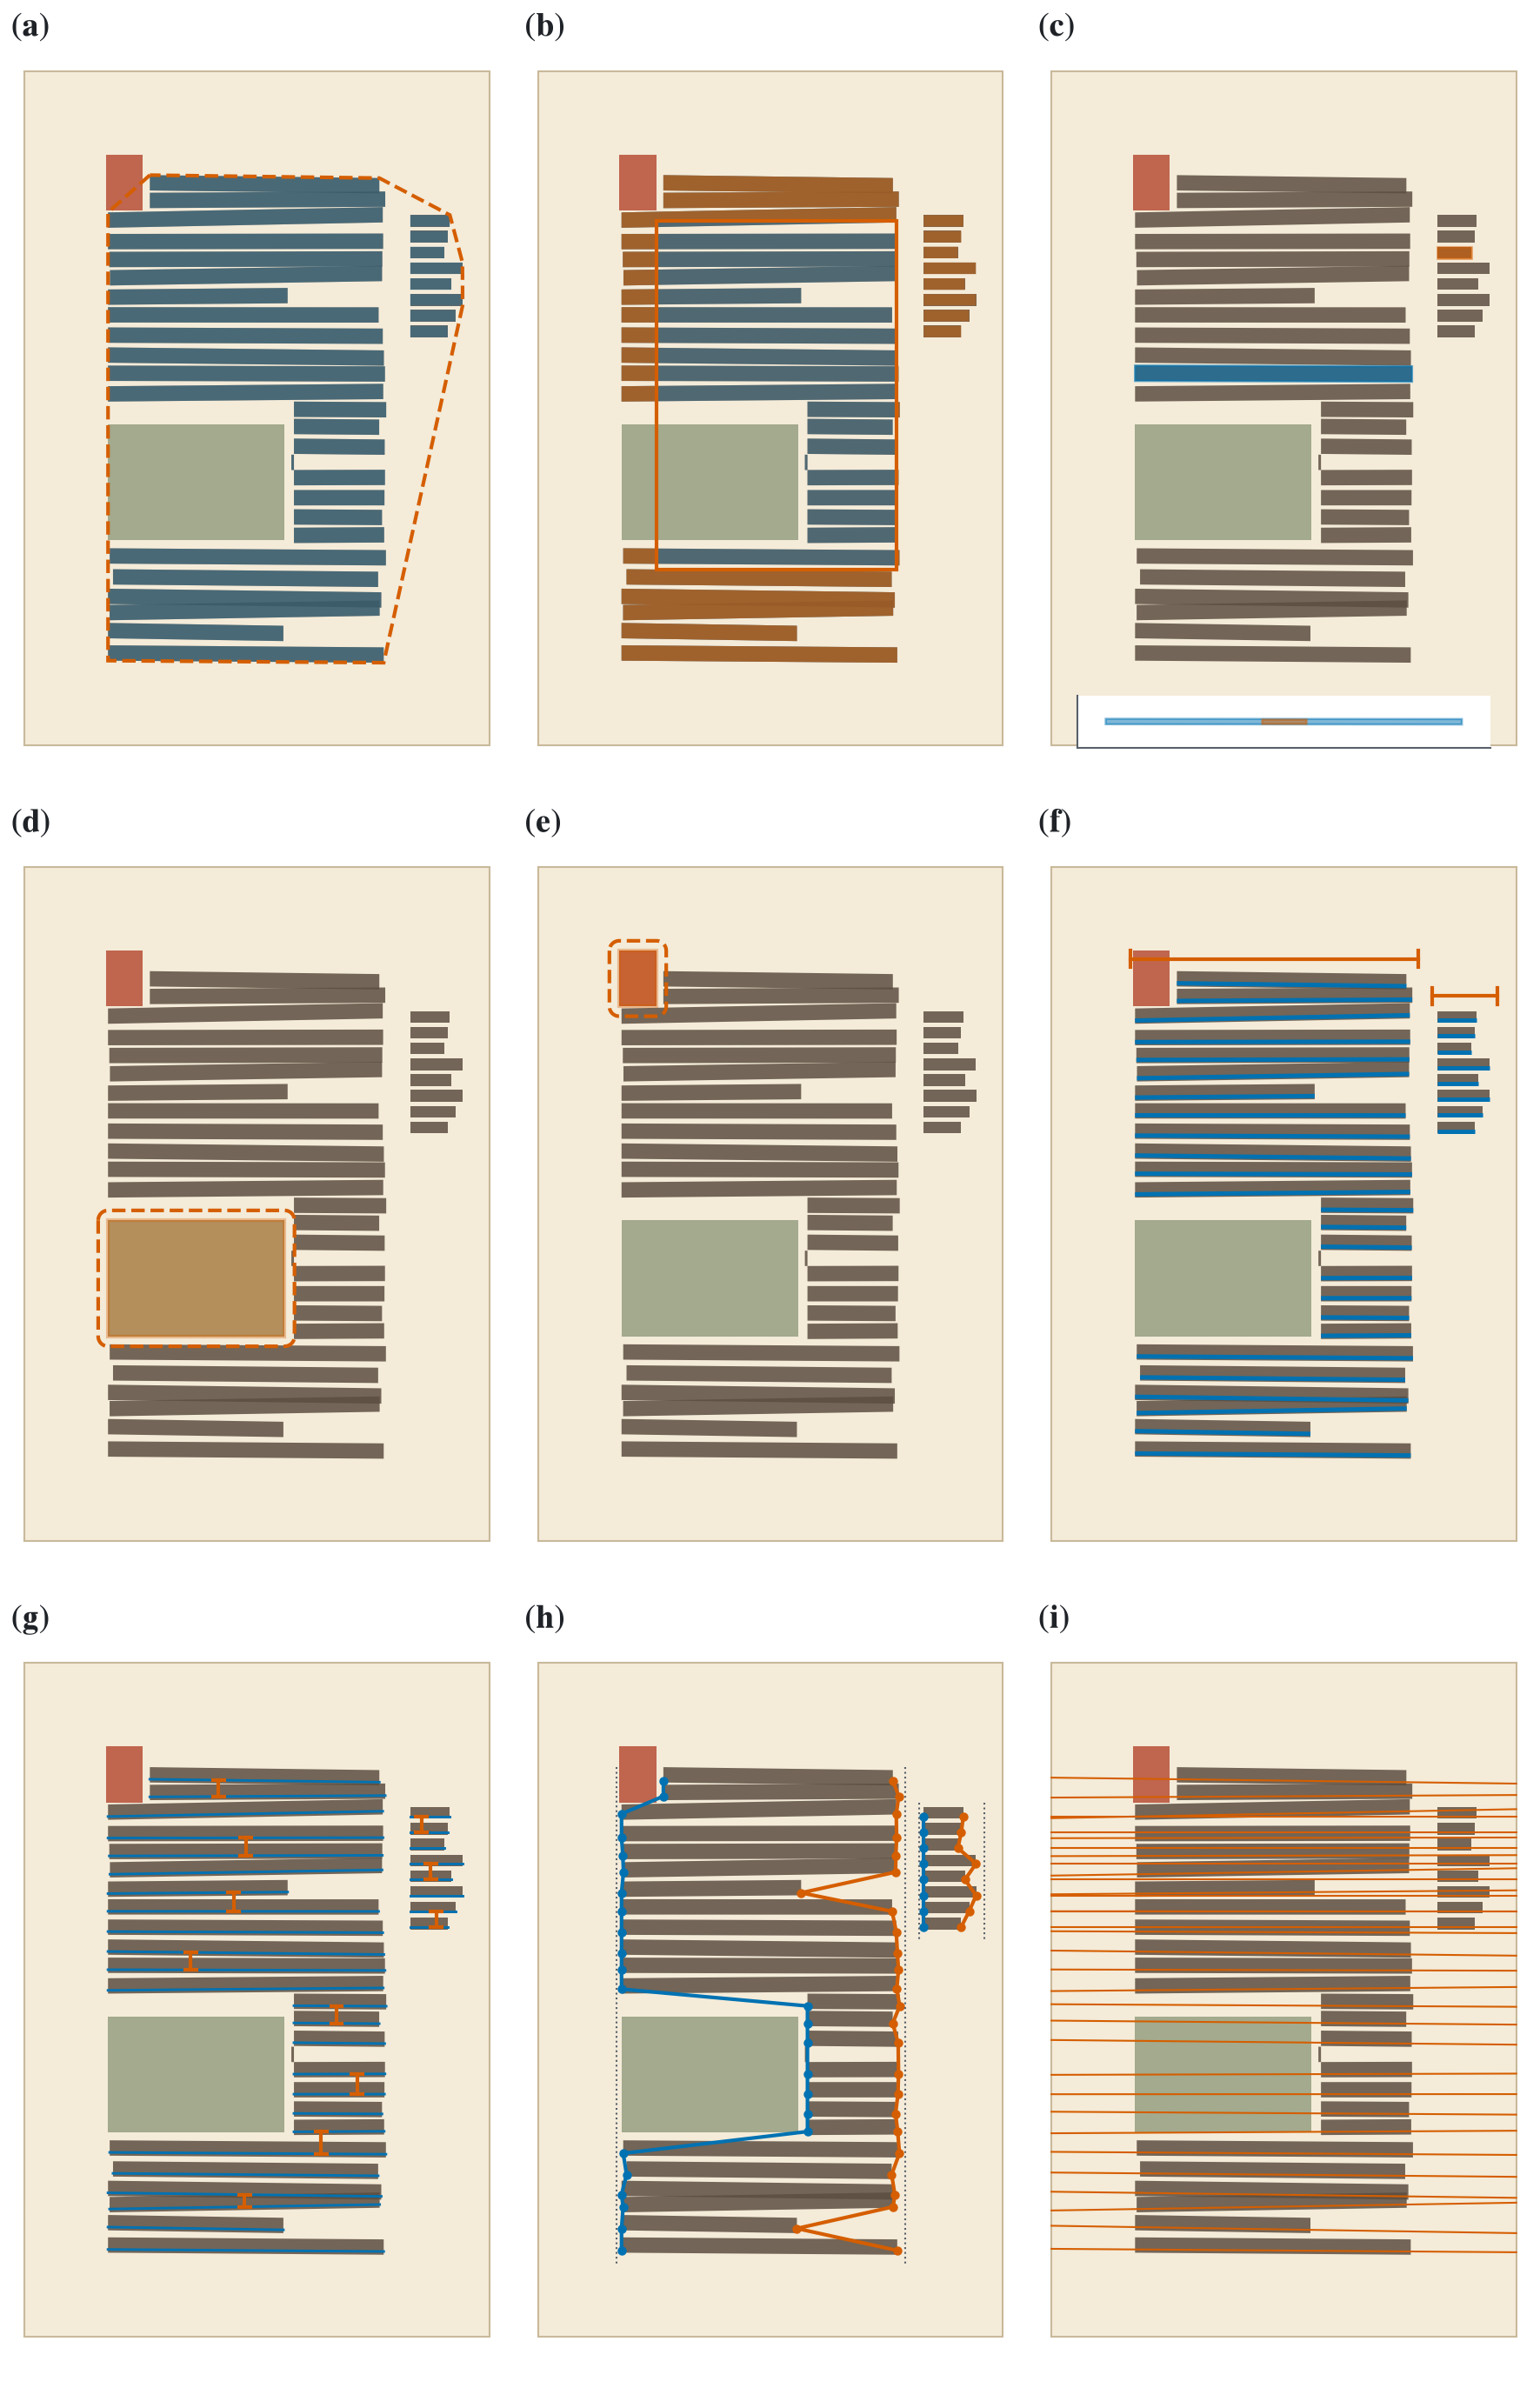
\includegraphics[width=15.00cm]{figures/geometry_features_on_schematic_page.png}
  \caption{The geometric features drawn on a made-up page: (a) the union of the line polygons (blue) and its convex hull (dashed) (\texttt{convexity} 0.541); (b) the written space (blue), the rectangle of its area and the folio's proportions centred on it, and the written space outside it (vermillion) (\texttt{outside\_ratio} 0.454); (c) the longest and the shortest line measured, and below, their polygons centred on each other (\texttt{dice\_median} 0.497); (d) the graphic zones (\texttt{graphic\_total\_area\_ratio} 0.066); (e) the drop capitals (\texttt{drop\_capital\_num\_isolated\_instances} 1); (f) the baselines measured (blue) and their zones' widths (\texttt{var\_coef} 0.275); (g) the baselines and, for every third pair, the distance between them (\texttt{max\_gap\_std} 0.052); (h) the lines' left (blue) and right (vermillion) ends, from line to line (\texttt{std\_right} 0.100); (i) each baseline's direction, drawn across the folio (\texttt{pairwise\_angle\_diff\_mean} 0.320).}
  \label{fig:geometry_features_on_schematic_page}
\end{figure}
